
\chapter{Task A}
\section{Environment description}
The environment is implemented as a weighted, un-directed graph, figure
\ref{fig:graph}.  The graph consist of Vertices(figure \ref{fig:vert}) and
Edges(figure \ref{fig:edge}) that is connected to each other.  By doing this we
can let the agent traverse the graph by itself using an implementation of the
shortest path algorithm as the heuristic for the A* algorithm to select the next
move to make. 

The environment also contains the possibility for marking edges as broken,
vertices as visited, and creating edges between Vertices.

\begin{figure}[h]\centering
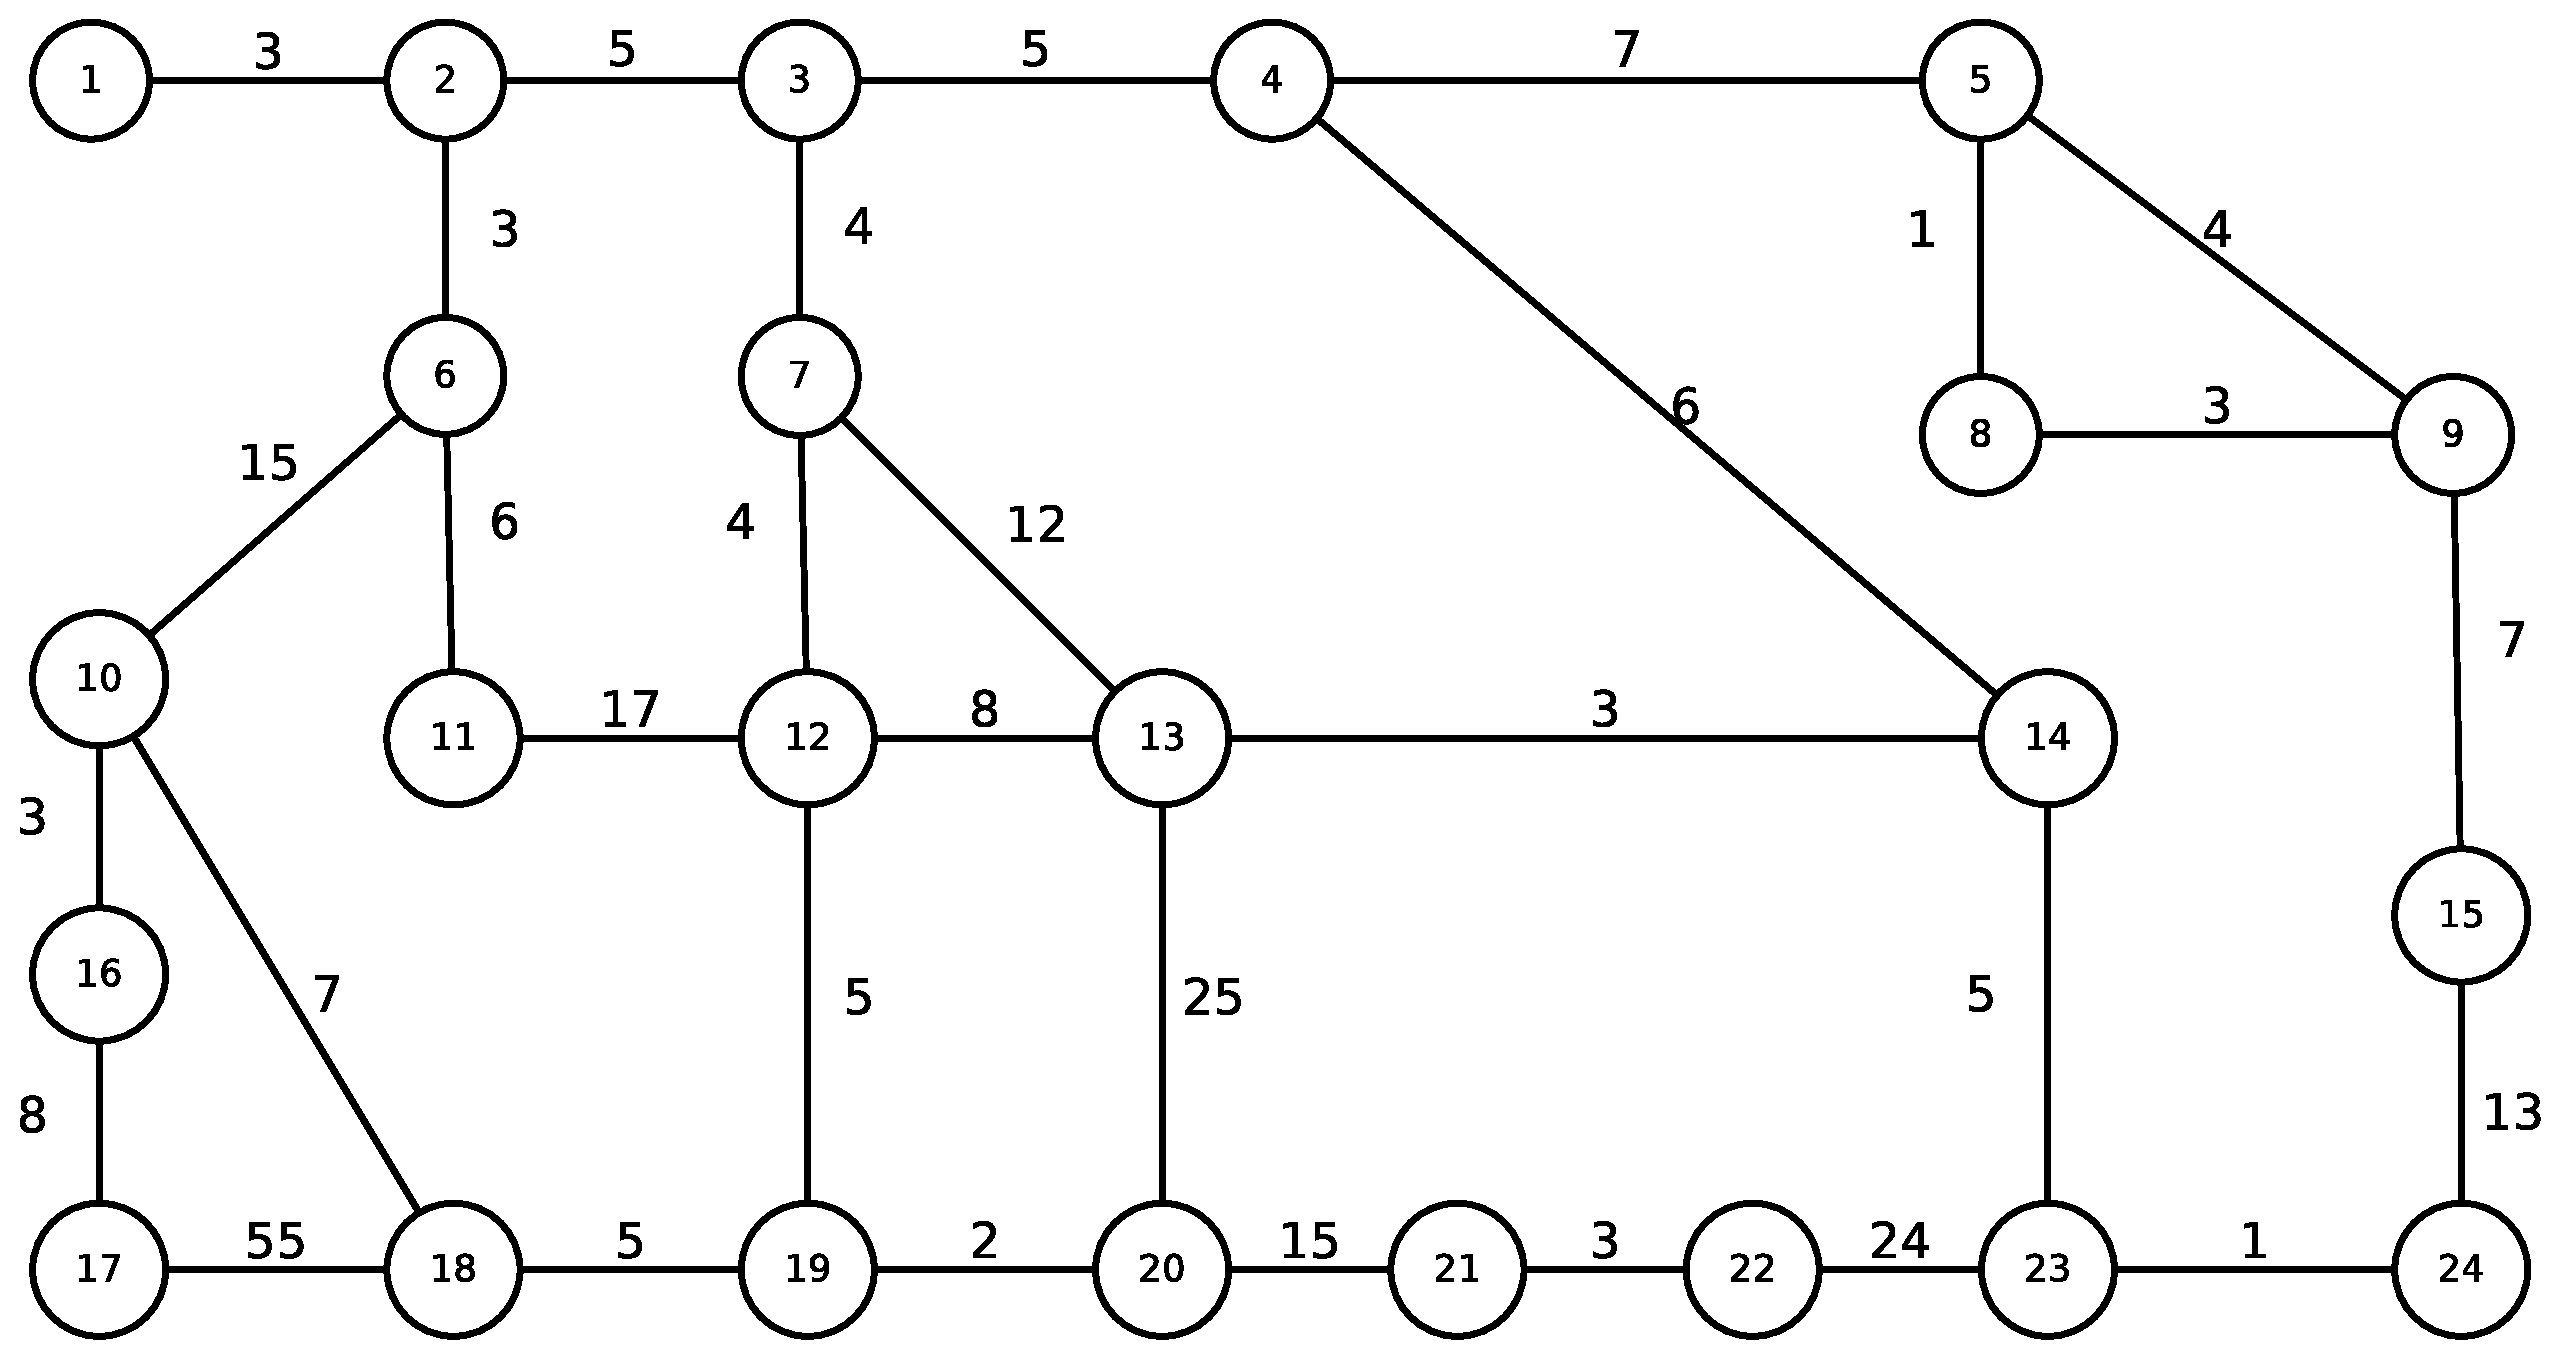
\includegraphics[ width={0.7\textwidth} ]{pictures/graph}
\caption{The environment - A non-directed graph with weighted edges.}
\label{fig:graph}
\end{figure}


\subsection{Creationism}
As the program starts up we read the file "vertice.lst" which contains a number
stating how many vertices are going to be in the graph. After reading this
integer we continue by creating the vertices and adding them to our Vertice
list.

The vertice list is built up using two elements to depict the start and end of
the list. The Vertice object, "vStart", is a dummy-element at the start of the
list. After this element all "real" elements follows.  Finally the last "real"
element is linked to the Vertice object "vTail", which represent the end of the
list.

The vertice list is represented in figure \ref{fig:vertlst}. The vStart object
is the start of the list, but holds no value other than a link to the first real
Vertice object. The "real" Vertices will hold different values describing its
state and information.

\begin{figure}[h]\centering
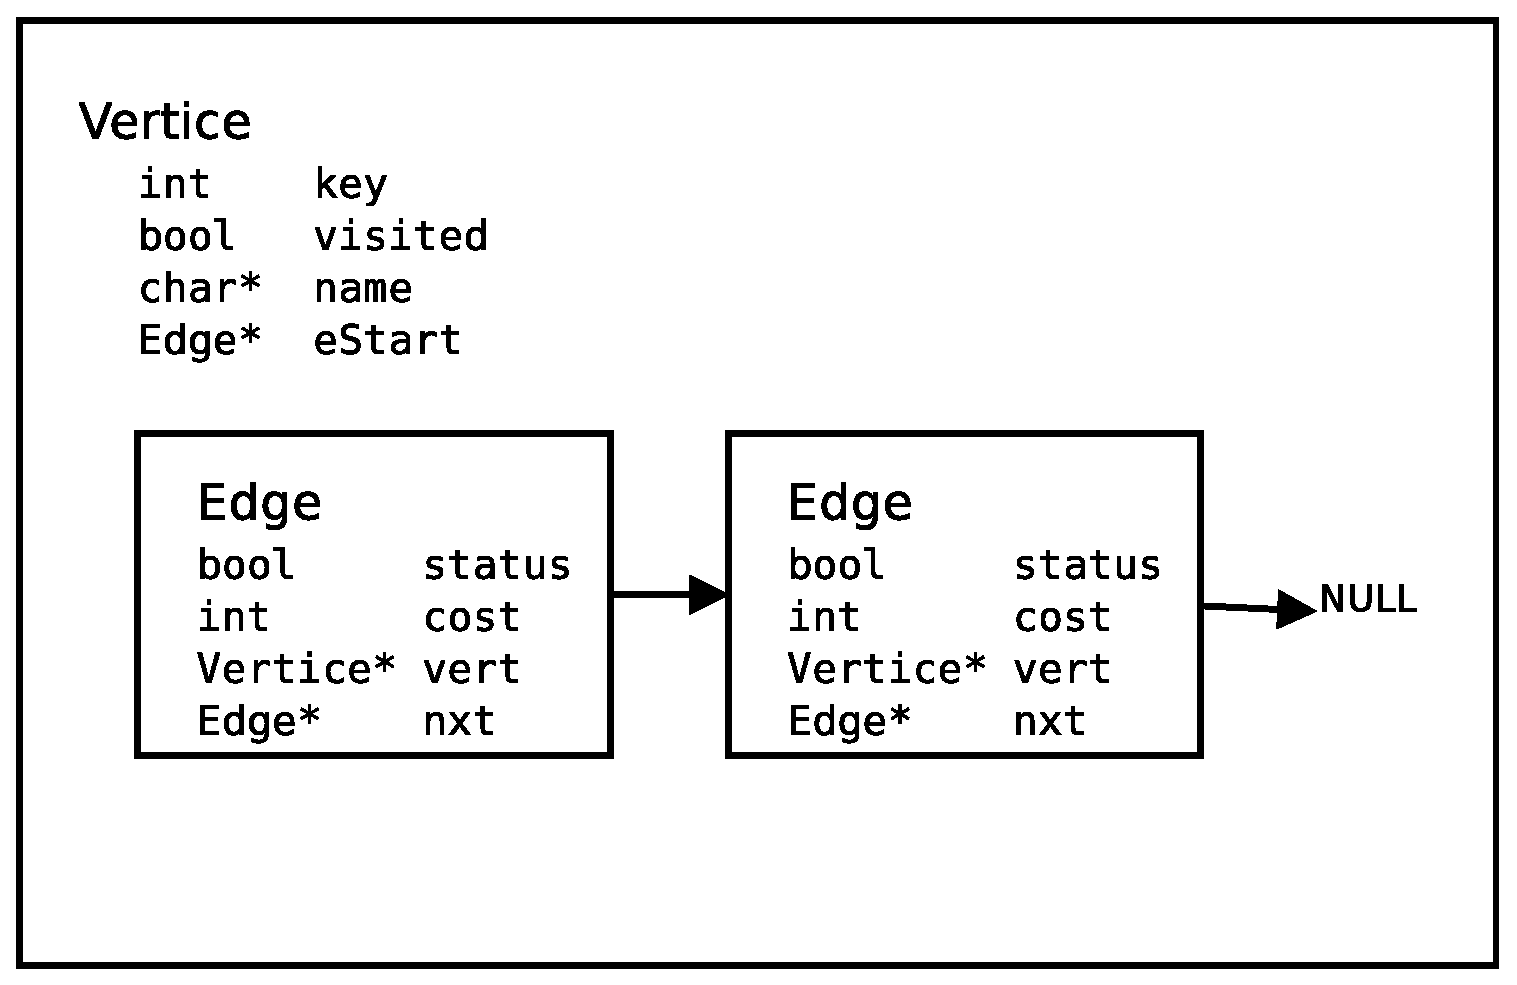
\includegraphics[ width={0.6\textwidth} ]{pictures/data_structure}
\caption{Illustration of the structure of a Vertice object}
\label{fig:vertlst}
\end{figure}

\subsection{Vertice}
\begin{description}
\item [key:]			This is an integer value holding the reference key to the
	Vertice. It is assigned automatically during creation of the vertice using an
	auto incremented counter starting at 1.  This is used to identify a specific
	Vertice in the graph and the vertice list.
\item [name:]			This is an unused variable and is assigned to NULL during
	creation. It is meant to hold a small text describing the name of the Vertice,
	and is usefull if it the graph represents a map or other things that could be
	assigned a description using a name tag.
\item [visited:]	This is a boolean describing wether or not the Vertice has
	been visited. It is not currently used, but could be used to mark a cell as
	visited during traversal.
\item [nxtVert:]	This is a pointer to a Vertice object. This will point to
	either the next Vertice in the list or to the vTail object which represents
	the end of the vertice list.  For vTail this link will link back to itsself.
\item [eStart:]		This is an Edge pointer which is on construction initialized
	to an Edge object that points to NULL.  This edge is the starting element for
	the list of Edges stemming from the current Vertice to adjacent vertices.
	eStart is however a dummy-element that points to the first actual edge in the
	list.
\end{description}
\begin{figure}\centering
	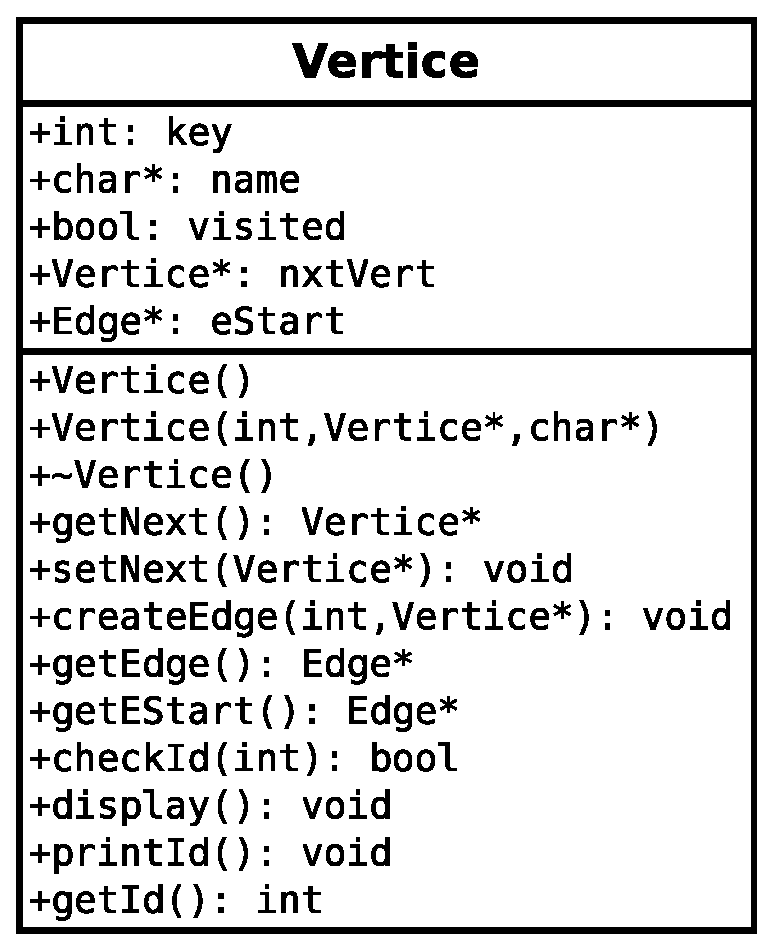
\includegraphics[ width={0.35\textwidth} ]{pictures/uml_vertice}
	\caption{UML description of a Vertice's variables and implemented functions}
	\label{fig:vert}
\end{figure}

\subsection{Edge}

\begin{description}
\item[status:]	This boolean value holds the status of the edge, which means 
	whether or not it	is traversable.  This could be used to update the 
	environment dynamically runtime.
\item[cost:]		This is the integer value representing the cost of traveling the
	edge from current vertice to the linked vertice.
\item[nxt:]			This is the a pointer to the next Edge in the edge list. The
	first edge in the list will be the dummy edge and the last element will point
	to NULL, which will result in a segfault if not handled properly.
\item[vert:]		This is a pointer to the linked Vertice in which the edge links
	to.
\end{description}

\begin{figure}[h]\centering
	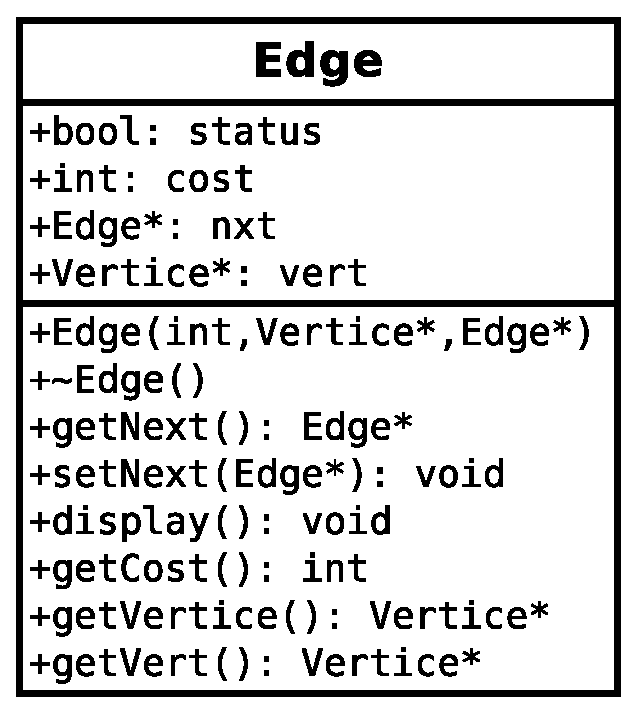
\includegraphics[ width={0.35\textwidth} ]{pictures/uml_edge}
	\caption{UML description of an Edge's variables and implemented functions}
	\label{fig:edge}
\end{figure}

\subsection{Vertice List}

\begin{figure}\centering
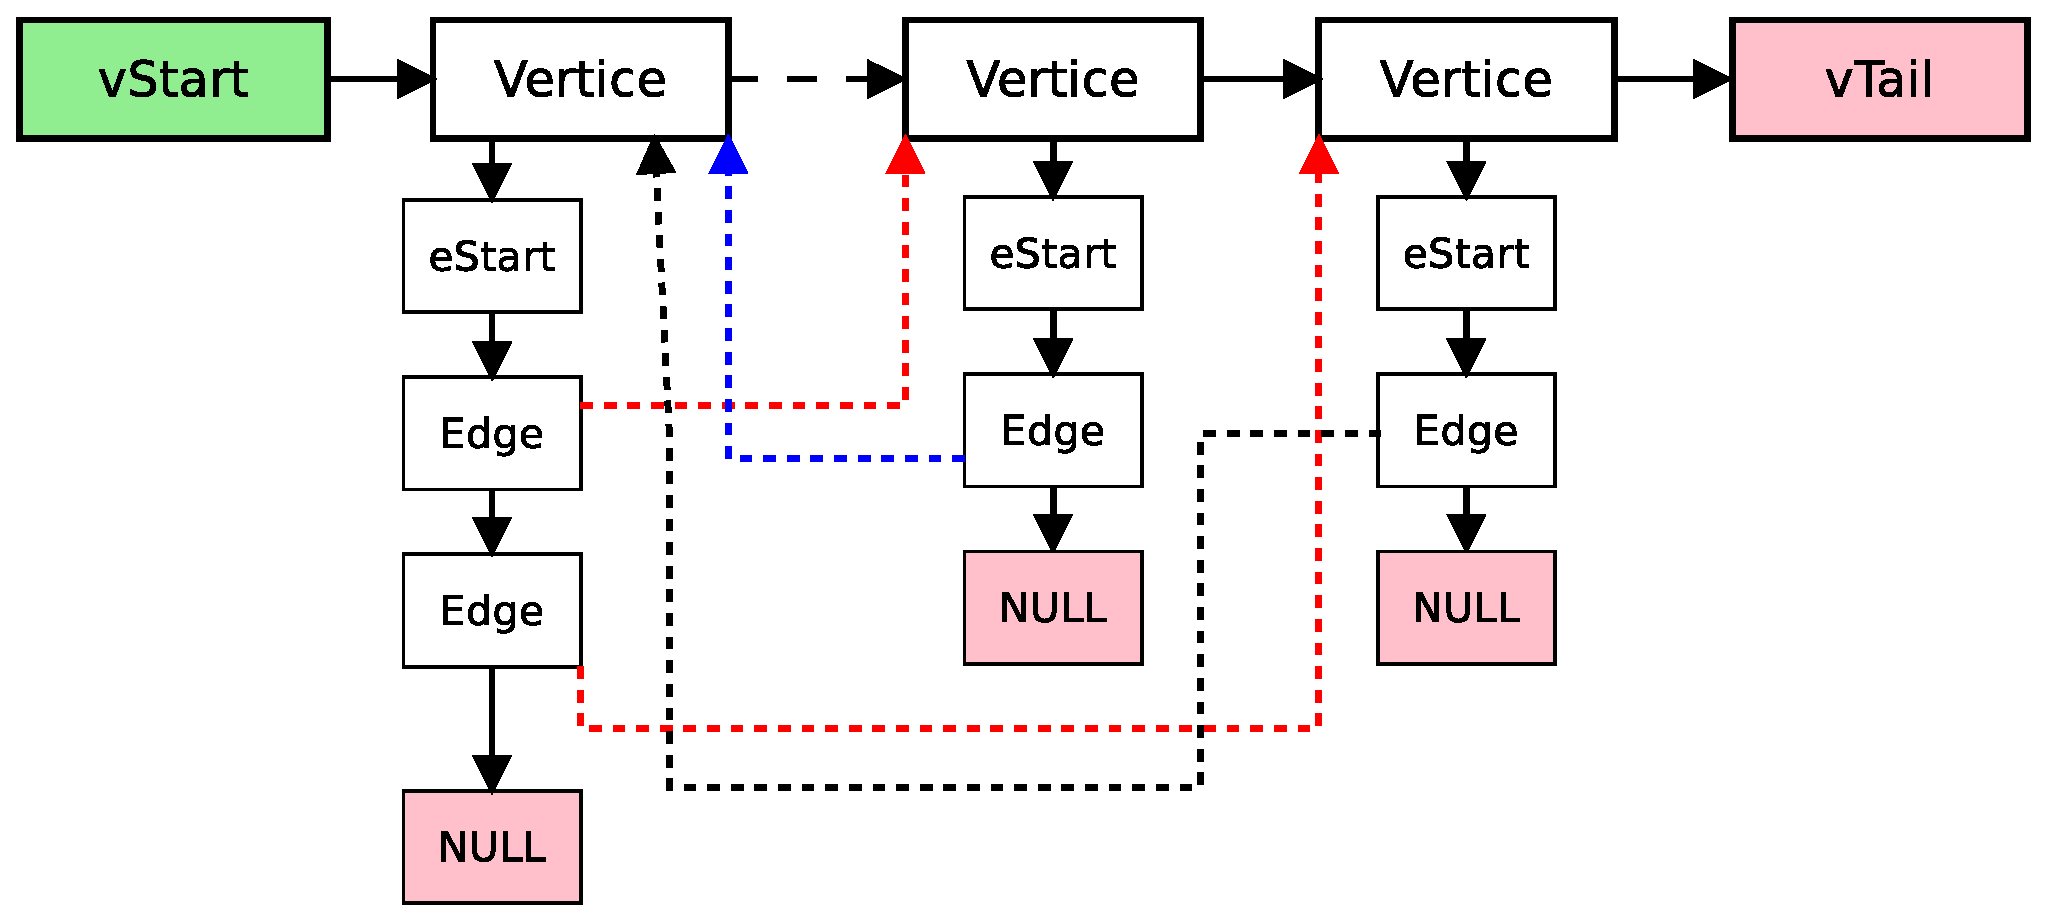
\includegraphics[ width={0.9\textwidth} ]{pictures/vertice_list}
\caption{Illustration of the list holding all the Vertices in the graph
environment}
\end{figure}


\subsection{Fringe List}


\begin{figure}\centering
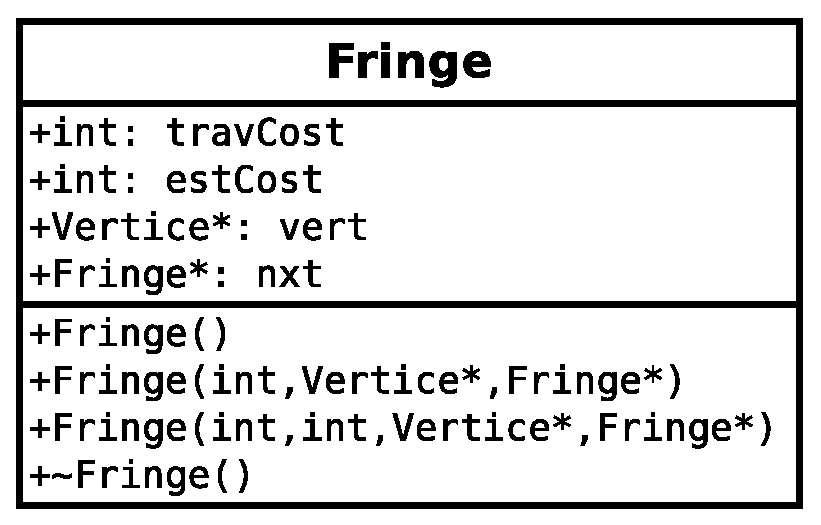
\includegraphics[ width={0.4\textwidth} ]{pictures/uml_fringe}
\caption{UML description of the Fringe object}
\end{figure}




\section{Agent - A* Tree Search}


\begin{figure}\centering
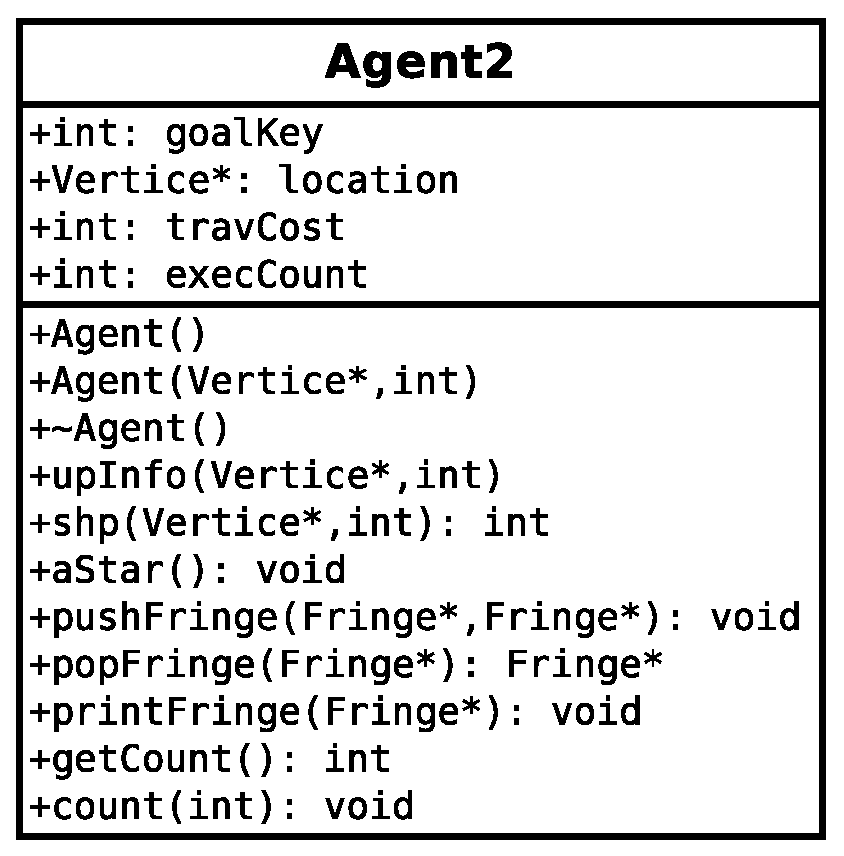
\includegraphics[ width={0.4\textwidth} ]{pictures/uml_agent2}
\caption{UML description of the Agent used for A* tree search}
\end{figure}


\section{A* Star Tree Search algorithm}

\begin{description}
\item[]
\end{description}

\begin{figure}
\centering
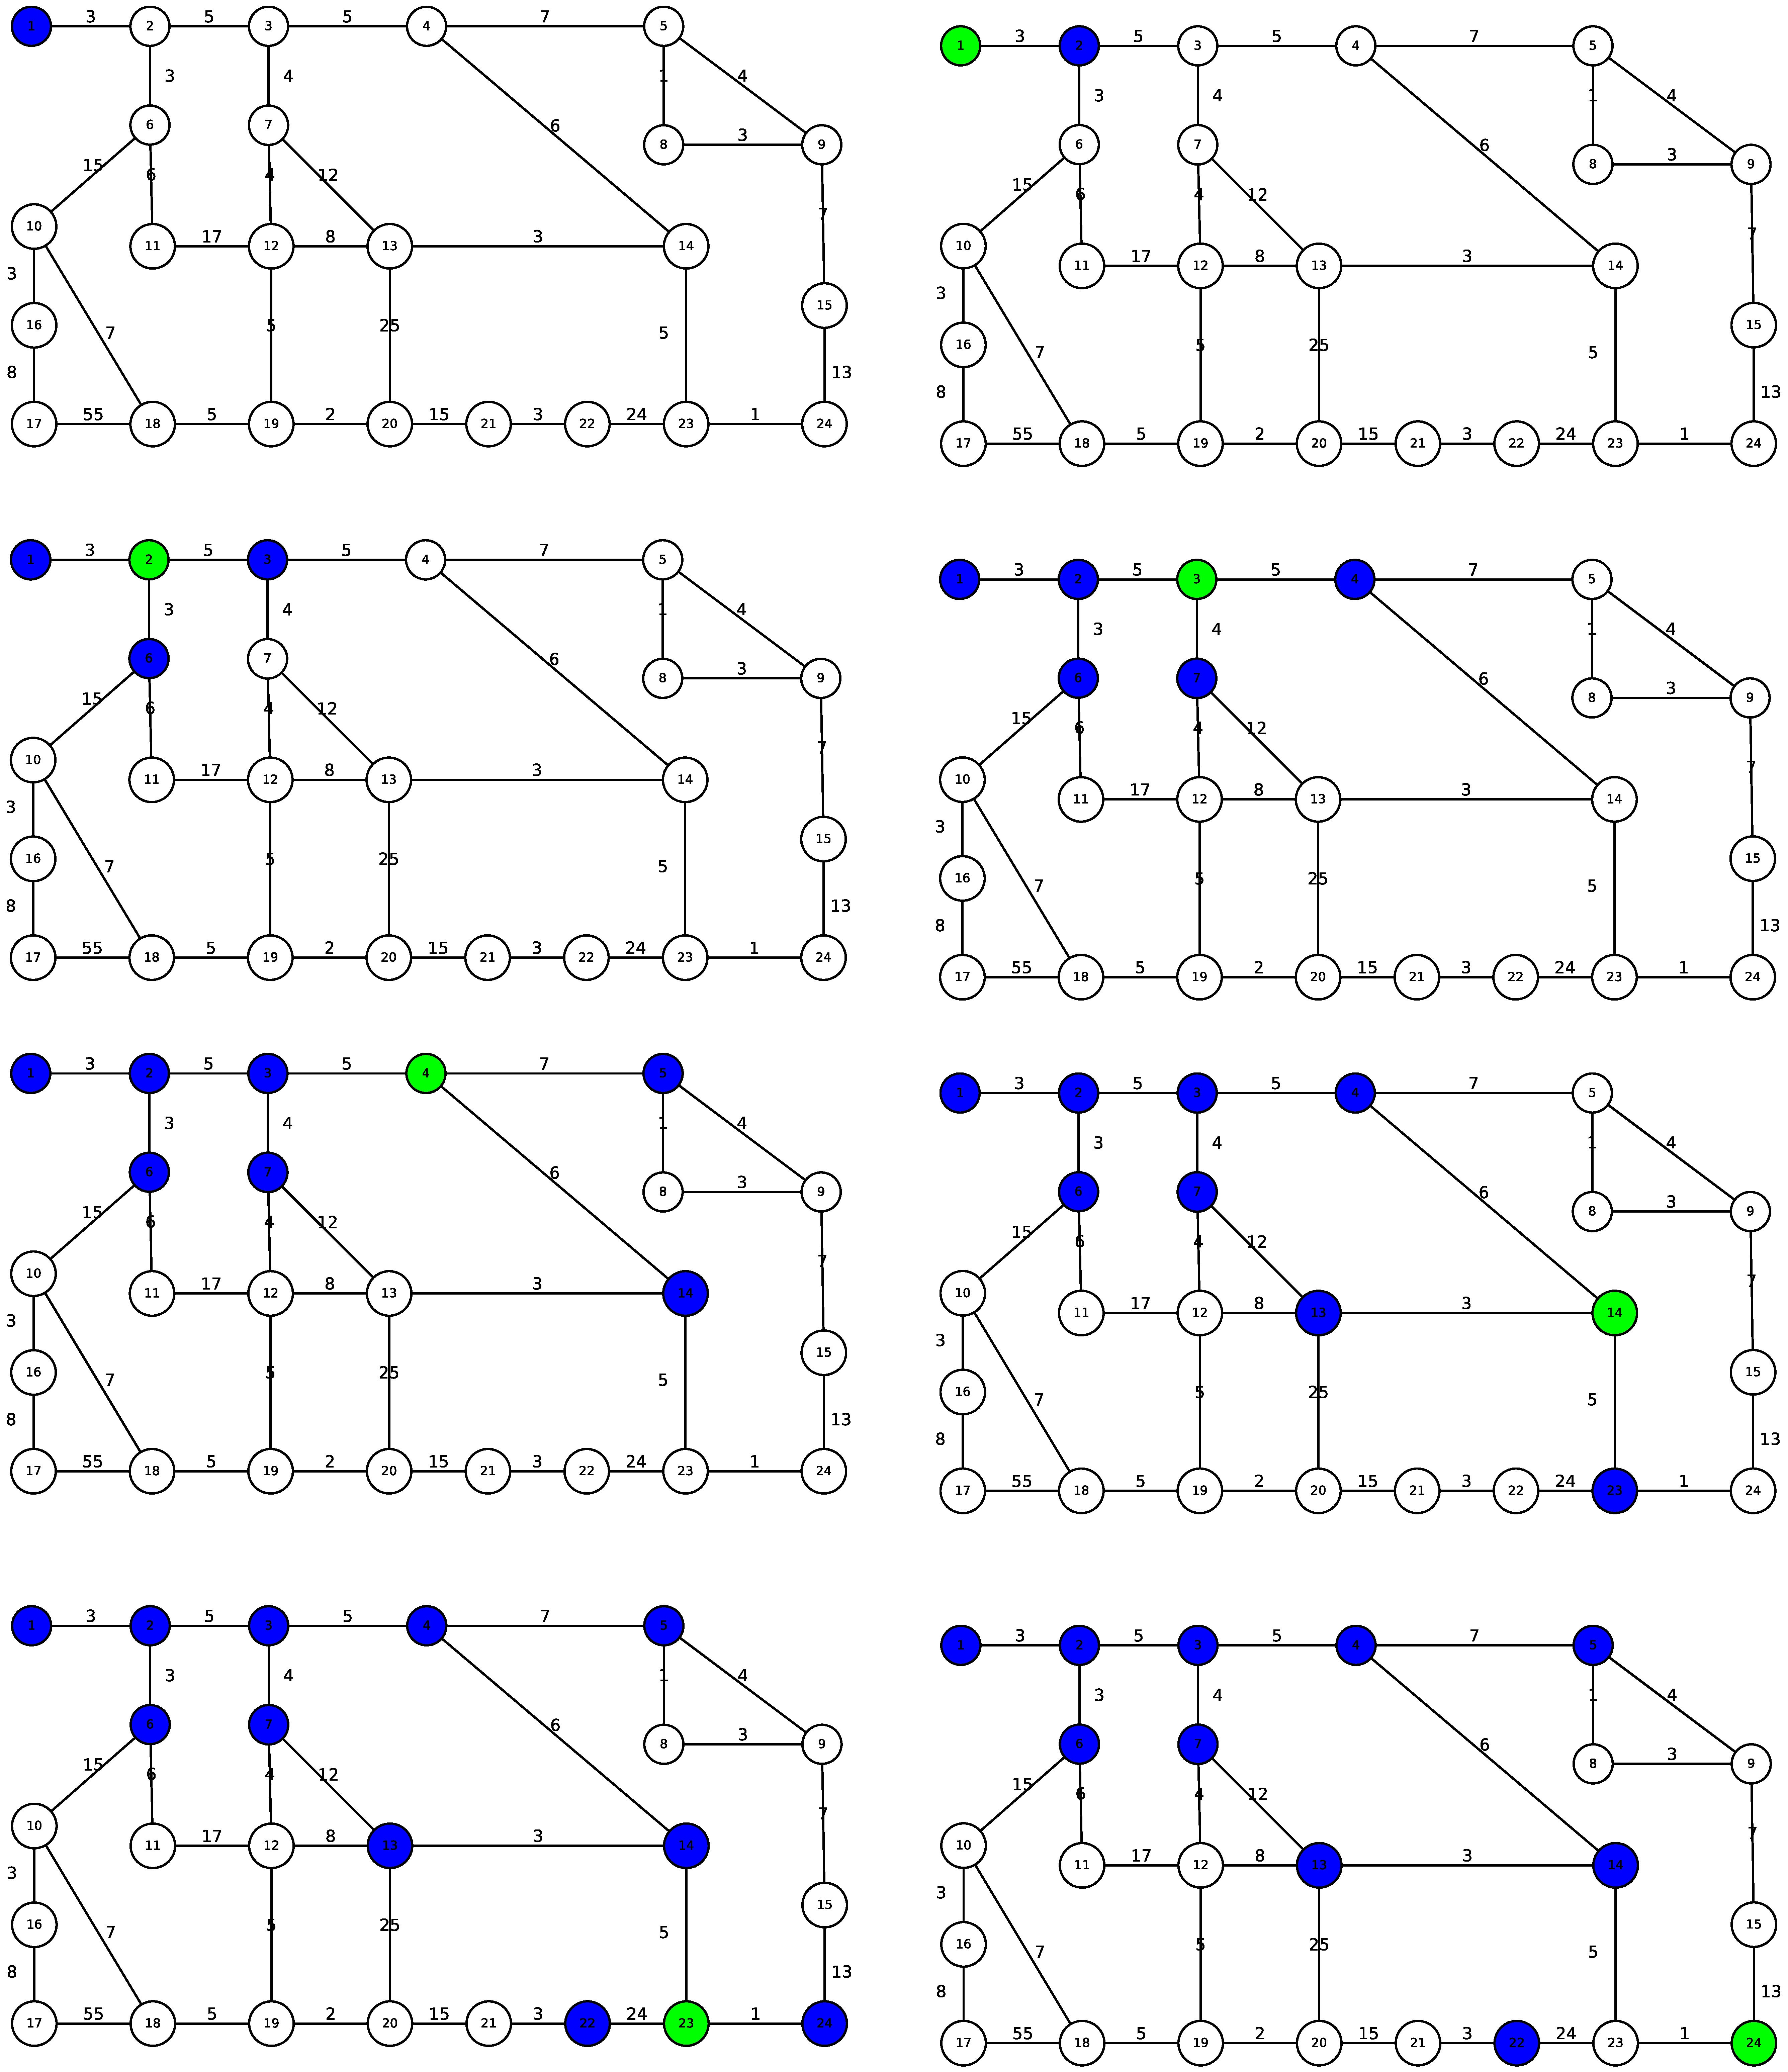
\includegraphics[ width={\textwidth} ]{pictures/tree_search}
\caption{A* star tree search algorithm}
\end{figure}


